\documentclass[a4paper,12pt]{extarticle}
\usepackage[utf8x]{inputenc}
\usepackage[T1,T2A]{fontenc}
\usepackage[russian]{babel}
\usepackage[hidelinks]{hyperref}
\usepackage{indentfirst}
\usepackage{listings}
\usepackage{color}
\usepackage{here}
\usepackage{array}
\usepackage{multirow}
\usepackage{graphicx}
\usepackage{subcaption} 
\usepackage{mathtools}

\usepackage{caption}
\renewcommand{\lstlistingname}{Программа} % заголовок листингов кода

\bibliographystyle{ugost2008ls}

\usepackage{listings}
\lstset{ %
extendedchars=\true,
keepspaces=true,
language=C,						% choose the language of the code
basicstyle=\footnotesize,		% the size of the fonts that are used for the code
numbers=left,					% where to put the line-numbers
numberstyle=\footnotesize,		% the size of the fonts that are used for the line-numbers
stepnumber=1,					% the step between two line-numbers. If it is 1 each line will be numbered
numbersep=5pt,					% how far the line-numbers are from the code
backgroundcolor=\color{white},	% choose the background color. You must add \usepackage{color}
showspaces=false				% show spaces adding particular underscores
showstringspaces=false,			% underline spaces within strings
showtabs=false,					% show tabs within strings adding particular underscores
frame=single,           		% adds a frame around the code
tabsize=2,						% sets default tabsize to 2 spaces
captionpos=t,					% sets the caption-position to top
breaklines=true,				% sets automatic line breaking
breakatwhitespace=false,		% sets if automatic breaks should only happen at whitespace
escapeinside={\%*}{*)},			% if you want to add a comment within your code
postbreak=\raisebox{0ex}[0ex][0ex]{\ensuremath{\color{red}\hookrightarrow\space}},
texcl=true,
inputpath=listings,                     % директория с листингами
}

\usepackage[left=2cm,right=2cm,
top=2cm,bottom=2cm,bindingoffset=0cm]{geometry}

%% Нумерация картинок по секциям
\usepackage{chngcntr}
\counterwithin{figure}{section}
\counterwithin{table}{section}

%%Точки нумерации заголовков
\usepackage{titlesec}
\titlelabel{\thetitle.\quad}
\usepackage[dotinlabels]{titletoc}

%% Оформления подписи рисунка
\addto\captionsrussian{\renewcommand{\figurename}{Рисунок}}
\captionsetup[figure]{labelsep = period}

%% Подпись таблицы
%\DeclareCaptionFormat{hfillstart}{\hfill#1#2#3\par}
%\captionsetup[table]{format=hfillstart,labelsep=newline,justification=centering,skip=-10pt,textfont=bf}

%% Путь к каталогу с рисунками
\graphicspath{{fig/}}

%% Внесение titlepage в учёт счётчика страниц
\makeatletter
\renewenvironment{titlepage} {
 \thispagestyle{empty}
}
\makeatother

\DeclarePairedDelimiter\abs{\lvert}{\rvert}%
\DeclarePairedDelimiter\norm{\lVert}{\rVert}%

\usepackage{amsmath}

\begin{document}	% начало документа

% Титульная страница
\begin{titlepage}	% начало титульной страницы

	\begin{center}		% выравнивание по центру

		\large Санкт-Петербургский политехнический университет Петра Великого\\
		\large Институт прикладной математики и механики \\
		\large Кафедра <<Прикладная математика>>\\[6cm]
		% название института, затем отступ 6см
		
		\huge Математическая статистика\\[0.5cm] % название работы, затем отступ 0,5см
		%\huge Методы оптимизации\\[0.5cm] % название работы, затем отступ 0,5см
		\large \textbf{Отчет по лабораторной работе №4}\\[5.1cm]
		%\large \textbf{Отчет по лабораторной работе \\``Решение задач одномерной минимизации ``}\\[5.1cm]
		%\\[5cm]

	\end{center}


	\begin{flushright} % выравнивание по правому краю
		\begin{minipage}{0.25\textwidth} % врезка в половину ширины текста
			\begin{flushleft} % выровнять её содержимое по левому краю

				\large\textbf{Работу выполнил:}\\
				\large Колесник В.Н.\\
				\large {Группа:} 3630102/70201\\
				
				\large \textbf{Преподаватель:}\\
				\large к.ф.-м.н., доцент\\
				\large Баженов Александр Николаевич
				%\large Родионова Елена Александровна

			\end{flushleft}
		\end{minipage}
	\end{flushright}
	
	\vfill % заполнить всё доступное ниже пространство

	\begin{center}
	\large Санкт-Петербург\\
	\large \the\year % вывести дату
	\end{center} % закончить выравнивание по центру

\end{titlepage} % конец титульной страницы

\vfill % заполнить всё доступное ниже пространство


% Содержание
\renewcommand\contentsname{\centerline{Содержание}}
\tableofcontents
\newpage

\listoftables
\newpage

\listoffigures
\newpage

\section{Постановка задачи}
Даны данные из Африки и Арктики, полученные в результате флуоресцентной спектроскопии. Это матрицы эмиссии. Они имеют участки высокой интенсивности, возникающие в результате излучения Релея. \\
Необходимо программно вырезать эти участки, посчитать интегралы по заданным зонам в разных пробах и составить гистограммы интенсивностей отдельно для проб Африки и Арктики.

\section{Теория}
\subsection{Компоненты флуоресценции}
Заданны следующие группы:
\begin{table}[!ht]
	\centering
		\begin{tabular} {|c|c|c|c|}
			\hline
			$E_{x_max}(nm)$ & $E_{m_max}(nm)$ & Тип компонента & Буквенное обозначение \\ \hline
			 320-350 & 420-480 & Humic-like & C \\ \hline
			 250-260 & 380-480 & Humic-like & A \\ \hline
			 310-320 & 380-420 & Marine Humic-like & M \\ \hline
			 270-280 & 300-320 & Tyrosine-like, Protein-like & B \\ \hline
			 270-280 & 320-350 & Tryptophane-like, Protein-like or phenol-like & T \\ \hline
		\end{tabular}
		\caption{Компоненты флуоресценции}
\end{table}

\section{Реализация}
Работа выполнена с помощью встроенных средств языка программирования R в среде разработки RStudio. Для работы с данными использовалась библиотека EEM. Исходный код работы приведён в приложении.\\
\\
Рассмотрим обработку данных на примере проб 1701 из Арктики и $1.1\_70$ из Африки. Визуально их можно представить так:
\begin{figure}[!htb]
    \centering
    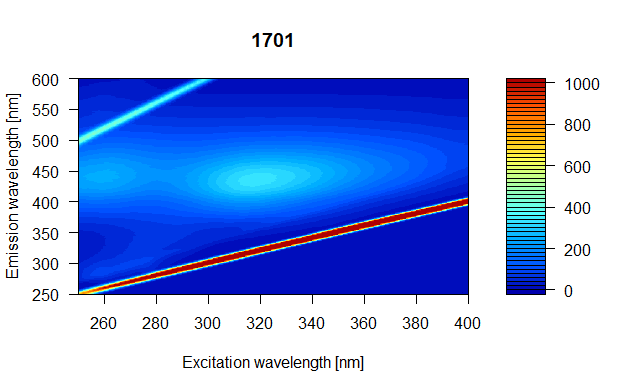
\includegraphics[width=0.5\textwidth]{fig/Arctic_1.png}
    \caption{Арктика. Проба 1701}
\end{figure}
\begin{figure}[!htb]
    \centering
    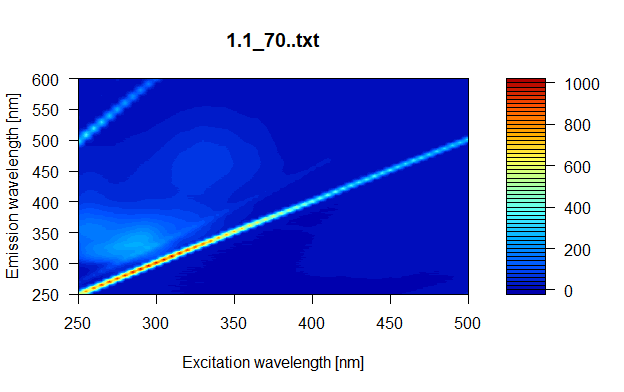
\includegraphics[width=0.5\textwidth]{fig/Africa_1.png}
    \caption{Африка. Проба $1.1\_70$}
\end{figure}
\newpage
Обработаем их с помощью метода delScattering2 библиотеки EEM. Получим:
\begin{figure}[!htb]
    \centering
    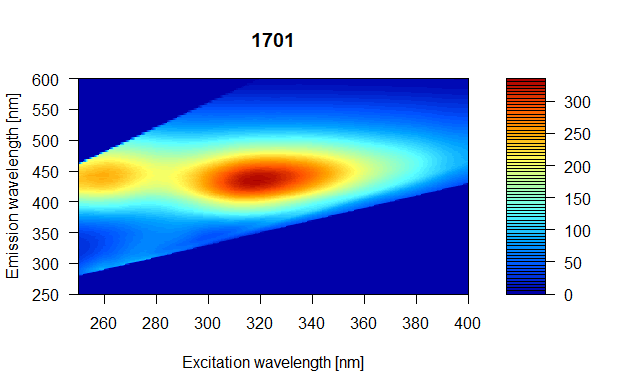
\includegraphics[width=0.5\textwidth]{fig/Arctic_2.png}
    \caption{Арктика. Проба 1701}
\end{figure}
\begin{figure}[!htb]
    \centering
    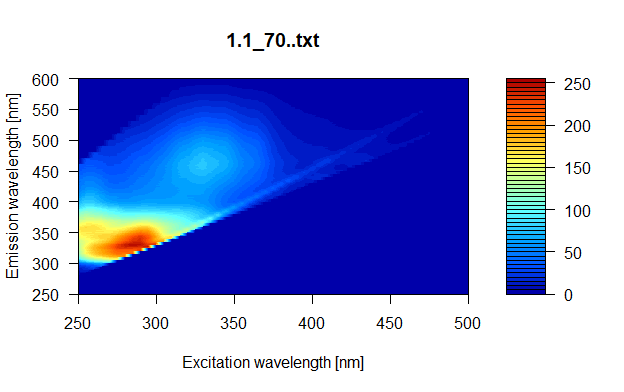
\includegraphics[width=0.5\textwidth]{fig/Africa_2.png}
    \caption{Африка. Проба $1.1\_70$}
\end{figure}
\newpage
Для получения компонент флуоресценции используем метод cutEEM. Полученные участки можно представить так:
 \begin{figure}[!htb]
    \centering
    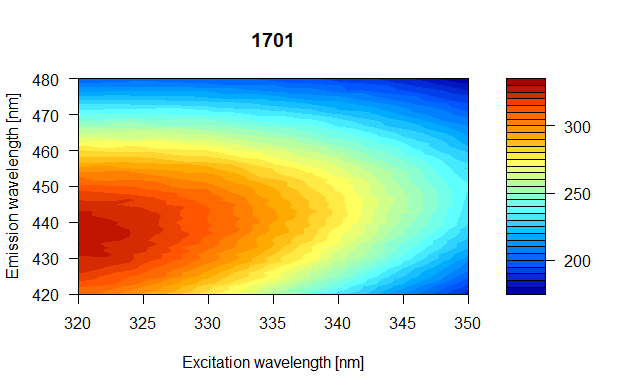
\includegraphics[width=0.5\textwidth]{fig/Arctic_3_C.png}
    \caption{Арктика. Проба 1701. C}
\end{figure}
 \begin{figure}[!htb]
    \centering
    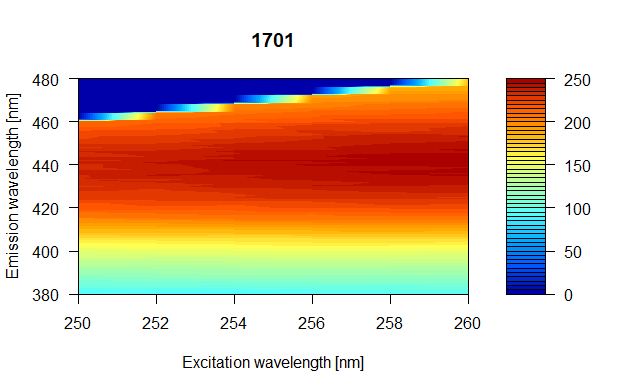
\includegraphics[width=0.5\textwidth]{fig/Arctic_3_A.png}
    \caption{Арктика. Проба 1701. A}
\end{figure}
 \begin{figure}[!htb]
    \centering
    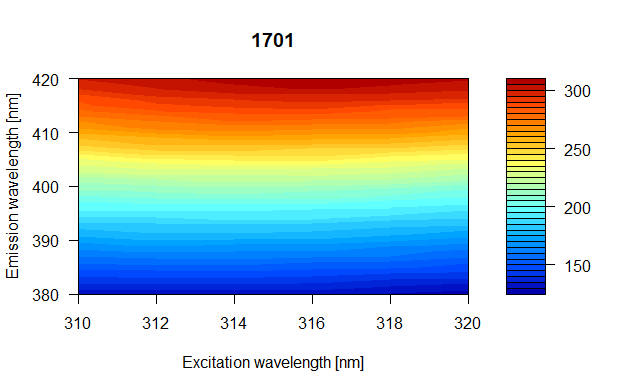
\includegraphics[width=0.5\textwidth]{fig/Arctic_3_M.png}
    \caption{Арктика. Проба 1701. M}
\end{figure}
\newpage
 \begin{figure}[!htb]
    \centering
    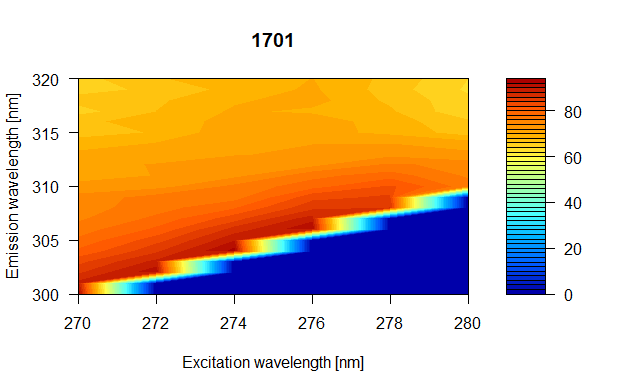
\includegraphics[width=0.5\textwidth]{fig/Arctic_3_B.png}
    \caption{Арктика. Проба 1701. B}
\end{figure}
 \begin{figure}[!htb]
    \centering
    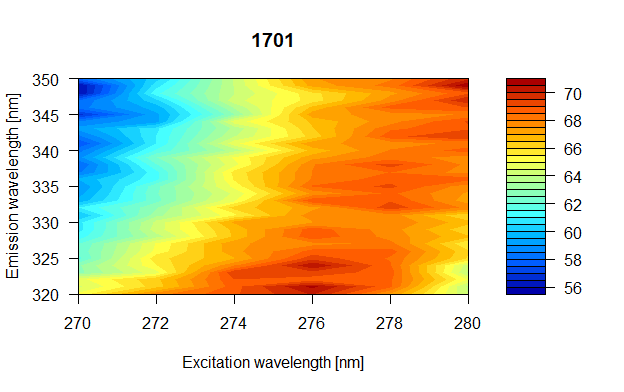
\includegraphics[width=0.5\textwidth]{fig/Arctic_3_T.png}
    \caption{Арктика. Проба 1701. T}
\end{figure}

 \begin{figure}[!htb]
    \centering
    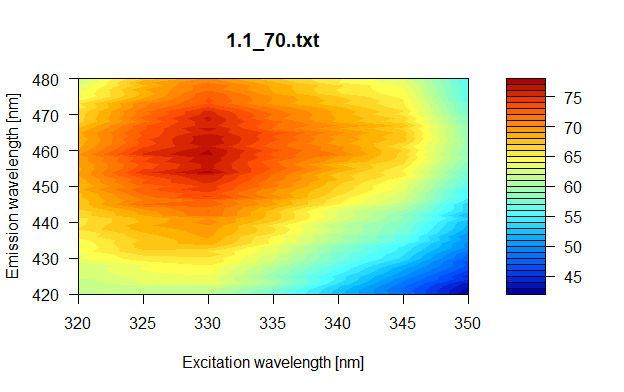
\includegraphics[width=0.5\textwidth]{fig/Africa_3_C.png}
    \caption{Африка. Проба $1.1\_70$. C}
\end{figure}
\newpage
 \begin{figure}[!htb]
    \centering
    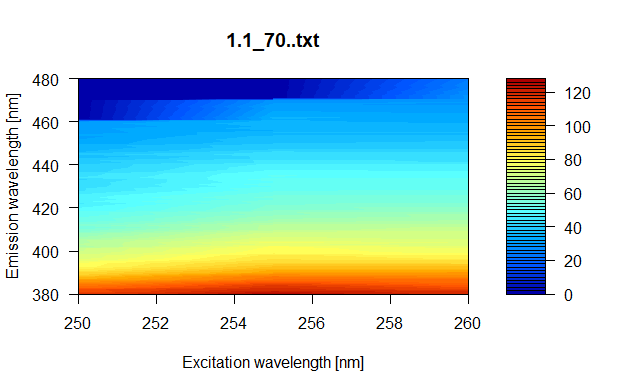
\includegraphics[width=0.5\textwidth]{fig/Africa_3_A.png}
    \caption{Африка. Проба $1.1\_70$. A}
\end{figure}
 \begin{figure}[!htb]
    \centering
    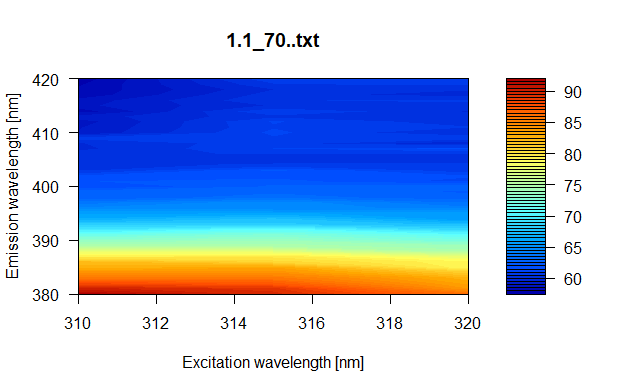
\includegraphics[width=0.5\textwidth]{fig/Africa_3_M.png}
    \caption{Африка. Проба $1.1\_70$. M}
\end{figure}
 \begin{figure}[!htb]
    \centering
    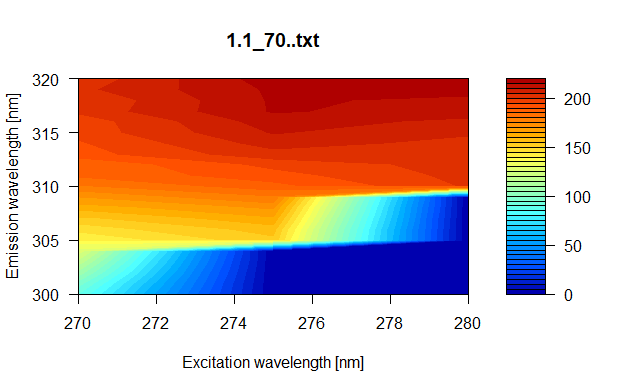
\includegraphics[width=0.5\textwidth]{fig/Africa_3_B.png}
    \caption{Африка. Проба $1.1\_70$. B}
\end{figure}
\newpage
 \begin{figure}[!htb]
    \centering
    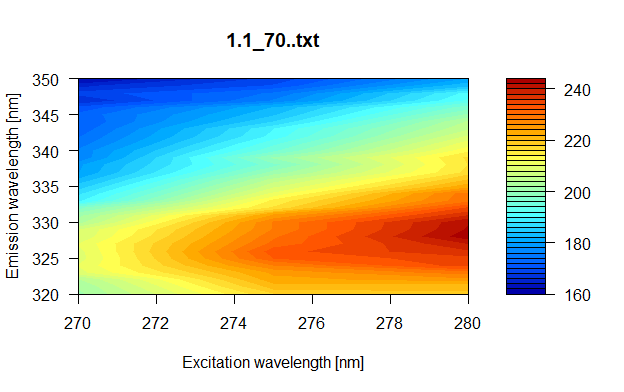
\includegraphics[width=0.5\textwidth]{fig/Africa_3_T.png}
    \caption{Африка. Проба $1.1\_70$. T}
\end{figure}
Значения интегралов по группам для этих 2 проб представлены в таблице:
\begin{table}[!ht]
	\centering
		\begin{tabular} {|c|c|c|c|c|c|}
			\hline
			Проба & C & A & M & B & T \\ \hline
			Арктика. 1701 & 254511 & 106220 & 53529 & 7156 & 12151 \\ \hline 
			Африка. $1.1\_70$ & 27637 & 15902 & 8280 & 8848 & 18995 \\ \hline 
		\end{tabular}
		\caption{Арктика 1701. Африка $1.1\_70$}
\end{table}

\section{Результаты}
Полученные данные были почищены, по заданным группам для каждой пробы были посчитаны интегралы. Результаты представлены в гистограммах.

\begin{figure}[!htb]
    \centering
    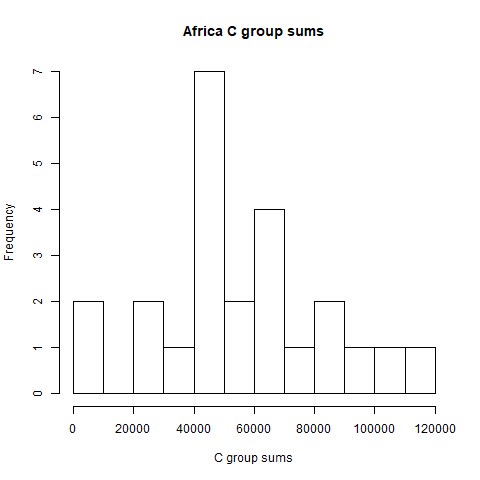
\includegraphics[width=0.5\textwidth]{fig/Africa_C.png}
    \caption{Африка. Группа C}
\end{figure}
\newpage
\begin{figure}[!htb]
    \centering
    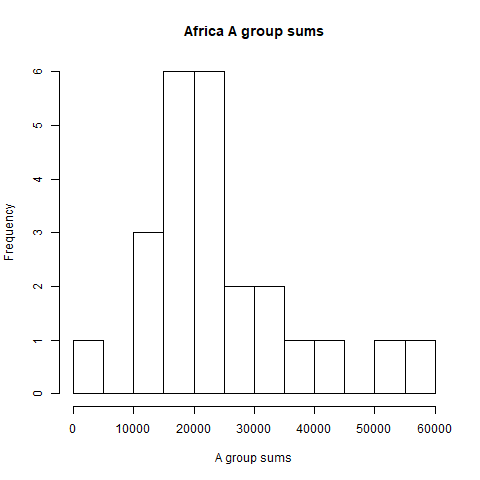
\includegraphics[width=0.5\textwidth]{fig/Africa_A.png}
    \caption{Африка. Группа A}
\end{figure}

\begin{figure}[!htb]
    \centering
    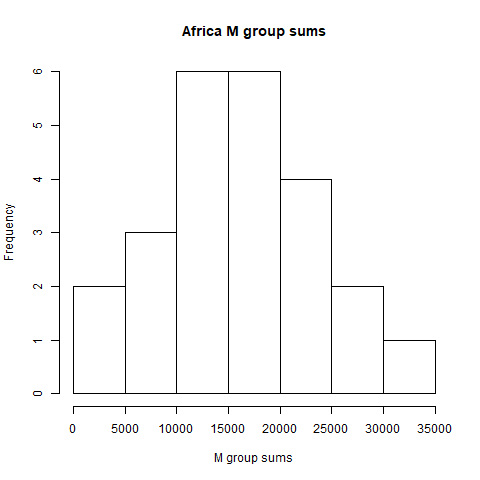
\includegraphics[width=0.5\textwidth]{fig/Africa_M.png}
    \caption{Африка. Группа M}
\end{figure}
\newpage
\begin{figure}[!htb]
    \centering
    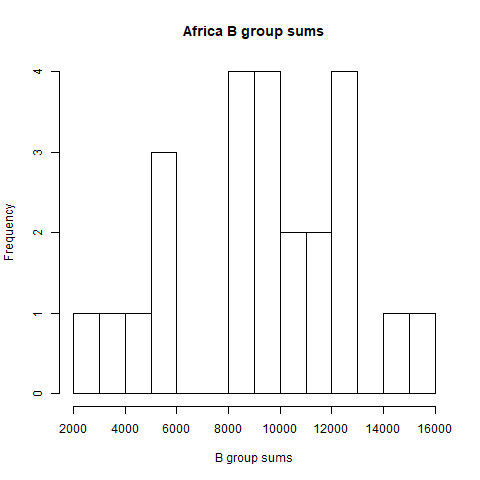
\includegraphics[width=0.5\textwidth]{fig/Africa_B.png}
    \caption{Африка. Группа B}
\end{figure}

\begin{figure}[!htb]
    \centering
    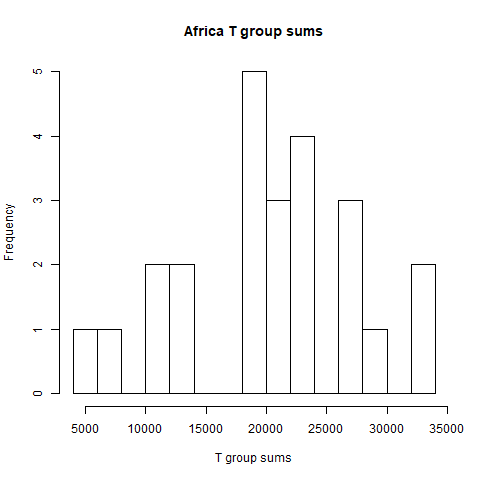
\includegraphics[width=0.5\textwidth]{fig/Africa_T.png}
    \caption{Африка. Группа T}
\end{figure}
\newpage
\begin{figure}[!htb]
    \centering
    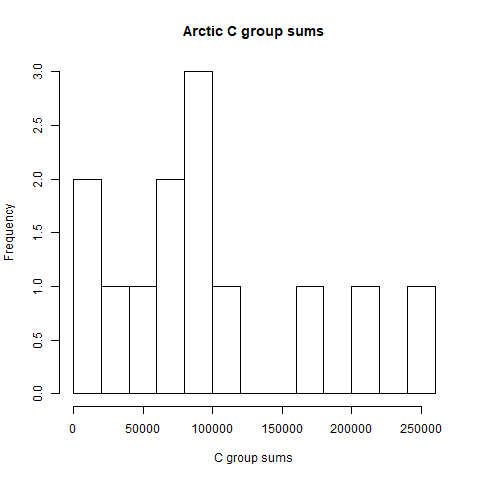
\includegraphics[width=0.5\textwidth]{fig/Arctic_C.png}
    \caption{Арктика. Группа C}
\end{figure}

\begin{figure}[!htb]
    \centering
    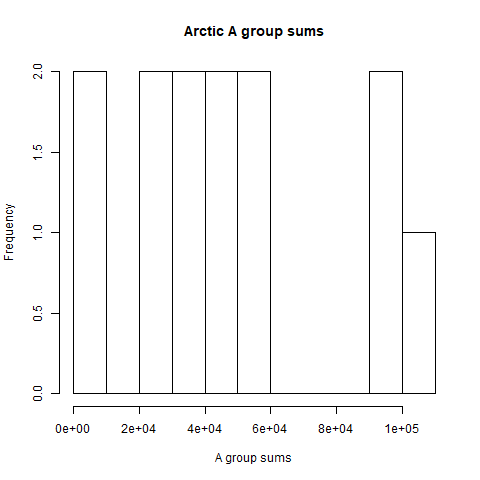
\includegraphics[width=0.5\textwidth]{fig/Arctic_A.png}
    \caption{Арктика. Группа A}
\end{figure}
\newpage
\begin{figure}[!htb]
    \centering
    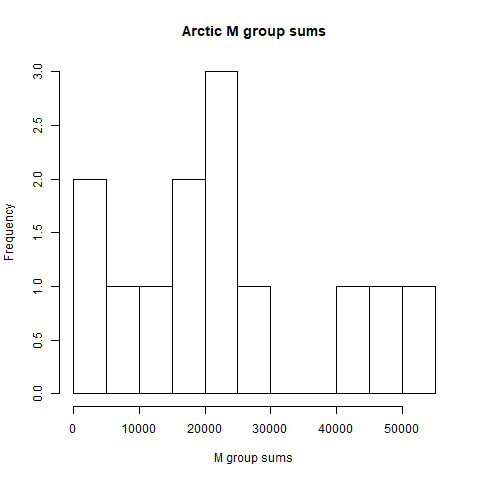
\includegraphics[width=0.5\textwidth]{fig/Arctic_M.png}
    \caption{Арктика. Группа M}
\end{figure}

\begin{figure}[!htb]
    \centering
    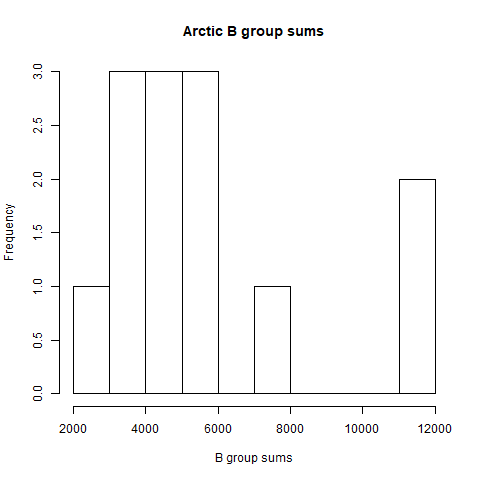
\includegraphics[width=0.5\textwidth]{fig/Arctic_B.png}
    \caption{Арктика. Группа B}
\end{figure}
\newpage
\begin{figure}[!htb]
    \centering
    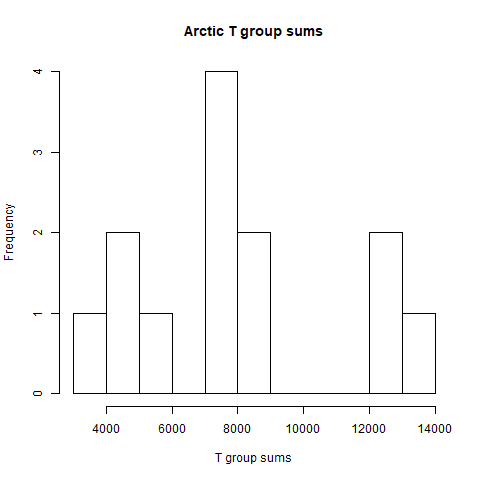
\includegraphics[width=0.5\textwidth]{fig/Arctic_T.png}
    \caption{Арктика. Группа T}
\end{figure}


\section{Приложения}
Репозиторий на Github с кодом лабораторной работы:\\
\url{https://github.com/VsevolodMelnikov/Math_Stat/tree/master/project}

\end{document}